\section{Tagging \& NE Chungking}

\begin{frame}
  \frametitle{Tagging \& NE Chunking}

  \begin{itemize}
  \item Text wird in einzelne Sätze aufgeteilt\\(\textbf{sentence tokenization})
  \item Sätze werden danach in Wörter und Satzzeichen zerlegt\\(\textbf{word tokenization})
  \item Wörtern und Satzzeichen werden Klassen zugeordnet\\(\textbf{pos
    tagging})
  \item Erkennung von bekannten Namen -- Städte, Personen, etc.\\(\textbf{named
    entity chunking})
  \item Die erzeugte Baumstruktur wird in eine flache Liste
    zurückgefüht, jedes \textit{named entity} erhält die Klasse \textit{NE}
  \end{itemize}
\end{frame}

\begin{frame}
  \frametitle{Beispiel}
  
  'A boy named Charlie Brown. And a car from Audi.'
  ~\\~\\
  \ensuremath {[}'A boy named Charlie Brown.', 'And a car from
  Audi.'\ensuremath{]}
  ~\\~\\
  \ensuremath{[}'A', 'boy', 'named', 'Charlie', 'Brown', '.', 'And', 'a', 'car',
  'from', 'Audi', '.'\ensuremath{]}
  ~\\~\\
  \ensuremath{[}('A', 'DT'), ('boy', 'NN'), ('named', 'VBN'), ('Charlie', 'NNP'),
  ('Brown', 'NNP'), ('.', '.'), ('And', 'CC'), ('a', 'DT'), ('car',
  'NN'), ('from', 'IN'), ('Audi', 'NNP'), ('.', '.')\ensuremath{]}
\end{frame}

\begin{frame}
  \frametitle{Beispiel}

  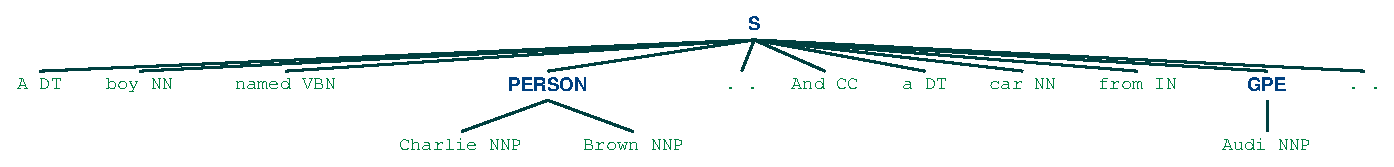
\includegraphics[scale=0.45]{img/ne_chunk_tree}
  ~\\~\\
  \ensuremath{[}('A', 'DT'), ('boy', 'NN'), ('named', 'VBN'),
  ('Charlie Brown', 'NE'), ('.', '.'), ('And', 'CC'), ('a', 'DT'),
  ('car', 'NN'), ('from', 'IN'), ('Audi', 'NE'), ('.', '.')\ensuremath{]}
\end{frame}

\begin{frame}
  \frametitle{Ergebnisse}

  \begin{itemize}
  \item Erkannt durch Hearst Patterns
    \begin{itemize}
    \item 2.716 Hypernyme
    \item 21.028 Hyponyme
    \end{itemize}

  \item Nach WordNet Filter
    \begin{itemize}
    \item 5 Hypernyme
    \item 6 Hyponyme
    \end{itemize}

  \end{itemize}
\end{frame}
